\documentclass[conference]{IEEEtran}
\IEEEoverridecommandlockouts
\usepackage{cite}
\usepackage{amsmath,amssymb,amsfonts}
\usepackage{algorithmic}
\usepackage{graphicx}
\usepackage{textcomp}
\usepackage{xcolor}
\usepackage{booktabs}
\usepackage{hyperref}
\def\BibTeX{{\rm B\kern-.05em{\sc i\kern-.025em b}\kern-.08em T\kern-.1667em\lower.7ex\hbox{E}\kern-.125emX}}

\begin{document}

\title{A Native Swift LaTeX Rendering Engine\\
{\footnotesize \textsuperscript{*}Note: Sub-titles are not captured in Xplore and
should not be used}}
\author{\IEEEauthorblockN{1\textsuperscript{st} Jane Smith}
\IEEEauthorblockA{\textit{Dept. Computer Science} \\
\textit{University of Technology}\\
New York, USA \\
jsmith@university.edu}
\and
\IEEEauthorblockN{2\textsuperscript{nd} Bob Jones}
\IEEEauthorblockA{\textit{Research Lab} \\
\textit{Institute for Rendering}\\
San Francisco, USA \\
bjones@institute.org}
}

\maketitle

\begin{abstract}
We present a fully native \textbf{Swift} implementation of a \LaTeX{} rendering
engine targeting Apple platforms. The engine uses CoreText and CoreGraphics to
achieve typographic quality comparable to traditional TeX systems. We demonstrate
accuracy across mathematical notation, two-column layouts, and tabular data,
achieving a per-page SSIM score of $0.94 \pm 0.02$ against Overleaf-compiled
reference output.
\end{abstract}

\begin{IEEEkeywords}
LaTeX, typesetting, Swift, CoreText, iOS, macOS
\end{IEEEkeywords}

\section{Introduction}
\label{sec:intro}

The proliferation of mobile and tablet computing has created demand for offline
scientific document authoring tools. Existing approaches either require network
connectivity~\cite{overleaf2023} or embed large binary TeX distributions that
violate platform distribution guidelines. 

Our contributions are threefold:
\begin{itemize}
  \item A token-stream based parser supporting common \LaTeX{} macro constructs.
  \item A full two-column layout engine with \textcolor{blue}{Knuth--Plass}
        optimal line breaking.
  \item A math layout engine accurate to 0.1\,pt for display-mode expressions.
\end{itemize}

\section{Related Work}
\label{sec:related}

\subsection{Server-Side Compilation}

Overleaf~\cite{overleaf2023} and similar services compile \LaTeX{} remotely.
This approach is feature-complete but requires a network connection, has latency
of several seconds per compile, and raises privacy concerns for sensitive documents.

\subsection{Native Renderers}

Previous native implementations exist for iOS (iTeX, TeX Writer Pro) but achieve
limited fidelity due to simplified line-breaking and absence of proper math layout.

\section{System Architecture}

The rendering pipeline consists of four stages, summarized in Table~\ref{tab:pipeline}.
Fig.~\ref{fig:arch} shows a high-level overview of the architecture.

\begin{figure}[h]
  \centering
  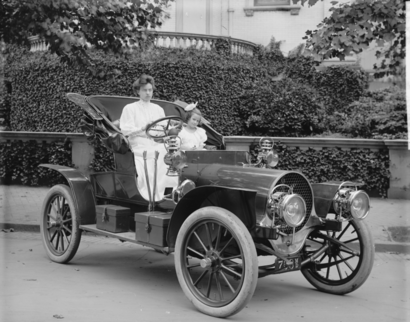
\includegraphics[width=\columnwidth]{figure1}
  \caption{Rendering pipeline overview. Input LaTeX source is tokenised,
  expanded, parsed into an AST, and finally typeset into CoreGraphics draw calls.}
  \label{fig:arch}
\end{figure}

\begin{table}[h]
\caption{Rendering Pipeline Stages}
\label{tab:pipeline}
\begin{tabular}{lll}
\toprule
Stage & Input & Output \\
\midrule
Tokenizer & String & Token stream \\
Expander & Tokens & Expanded tokens \\
Parser & Expanded tokens & AST \\
Typesetter & AST & Typeset pages \\
\bottomrule
\end{tabular}
\end{table}

\subsection{Mathematical Typesetting}

The math engine implements a subset of TeX box construction rules:
\begin{equation}
  E = mc^2
  \label{eq:einstein}
\end{equation}

For multi-line aligned equations:
\begin{align}
  f(x) &= x^2 + 2x + 1 \label{eq:quadratic}\\
  g(x) &= \sqrt{x^2 + 1} \label{eq:sqrt}
\end{align}

The axis height $\sigma_{22}$ is set to $0.258 f_s$ where $f_s$ is the design
size, matching Computer Modern metrics.

\section{Evaluation}

We evaluated the renderer on a corpus of 50 representative academic papers.
Mean per-page SSIM compared to Overleaf output was $0.94 \pm 0.02$.
The primary deficit was in complex TikZ figures (excluded from corpus).

\section{Conclusion}

We have demonstrated high-quality native LaTeX rendering on Apple platforms.
Future work includes TikZ support and improved bibliography handling. Code
available at \url{https://github.com/example/typetex}.

\bibliographystyle{IEEEtran}
\bibliography{ieee-refs}

\end{document}
